
\section{Following paths}

% specification
\paragraph{Specification}{
    Basically, the program should respect the rules below, extract from the assignment wording itself.
    \begin{itemize}
        \item Implement a program that interacts with the Kompai robot in MRDS.
        This involves implementing functions for reading the robot's sensors
        and controlling the robot's actuators.
        
        \item Implement a controller that enables the robot to follow a
        specified path given as a sequence of coordinates. Small divergences
        from the specified path are allowed, but the controller must be able to
        steer the robot back onto the path when divergences from the path occur.
        
        \item The controller must be able to successfully track a few test
        paths, without hitting walls and other obstacles. You may use these
        paths as examples, or record your own (see below).
        
        \item The program should include some means of displaying the time
        taken from start to finish. The start is defined as the moment the
        robot starts moving, and finish is defined as the moment the robot is
        within 1 meter of the last point in the path.
    \end{itemize}

}

% run the program

\paragraph{Run the program}{
    To run the program, first open MRDS and load the simulation used for the
 assignment. Then run the program from a shell like this : \texttt{\$ python
 follow\_the\_path.py <file>}. \texttt{<file>} must be a file containing a path
 to follow for the opened simulation and formatted in JSON.s
}

\paragraph{Follow the carrot}{
    There are several ways to make a robot following a given path. For this
assignment, as it was suggested, I decided to implement the algorithm
\textit{follow the carrot}. This simple algorithm is presented by Barton in
his PhD thesis\cite{thesis:barton}. The figure \ref{algo:base} takes over
this method.
}

\begin{figure}[!h]
    \begin{algorithmic}
        \ForAll{point in path}
            \State $position \gets \Call{getRobotRosition}$
            \While{$position \neq point$}
                \State $speeds \gets \Call{compute\_speeds(position, point)}$
                \State $\Call{setSpeeds}{speeds}$
                \State $position \gets \Call{getRobotRosition}$
            \EndWhile
        \EndFor
        \State $\Call{setSpeeds}{\{0, 0\}}$
    \end{algorithmic}
    
    \caption{
        \label{algo:base}
        \textit{Follow the carrot} algorithm
    }
\end{figure}

\paragraph{Speeds computation}{
    The functions called in this algorithm already exists and are designed to
control or to get data from the robot. But there is no way to compute the speeds,so I implemented the function \texttt{compute\_speeds} which computes
the angular and the linear speed of the robot regarding his position and the
target position. Only this two value are needed to move the robot around.
The computation is presented figure \ref{algo:speeds}. It is essentially about
using mathematical functions and tools.
}

\begin{figure}[!h]
    \begin{algorithmic}
     \Function{compute\_speeds}{robot, carrot}
        \State $distance \gets \sqrt{(carrot.x - robot.x)^{2} + (carrot.y - robot.y)^{2}}$
        \State $robot\_angle \gets \Call{getRobotSteering}$
        \State $carrot\_angle \gets \Call{atan2}{carrot.y - robot.x, carrot.x - robot.x}$
        \State $angle = carrot\_angle - robot\_angle$
        \State $angular\_speed = angle / 1$
        \State $linear\_speed \gets angular\_speed \times \frac{distance}{2 \times sin( angle )} $
        \State \Return $linear\_speed,~angular\_speed$
     \EndFunction
    \end{algorithmic}
    
    \caption{
        \label{algo:speeds}
        Algorithm to compute the speed to reach a target point
    }
\end{figure}

\begin{figure}[!h]
    \begin{center}
        % Graphic for TeX using PGF
% Title: /home/ens15/ens15bsf/edu/5dv121/lab1/report/src/figures/long_path.dia
% Creator: Dia v0.97.3
% CreationDate: Tue Oct 27 16:01:42 2015
% For: ens15bsf
% \usepackage{tikz}
% The following commands are not supported in PSTricks at present
% We define them conditionally, so when they are implemented,
% this pgf file will use them.
\ifx\du\undefined
  \newlength{\du}
\fi
\setlength{\du}{15\unitlength}
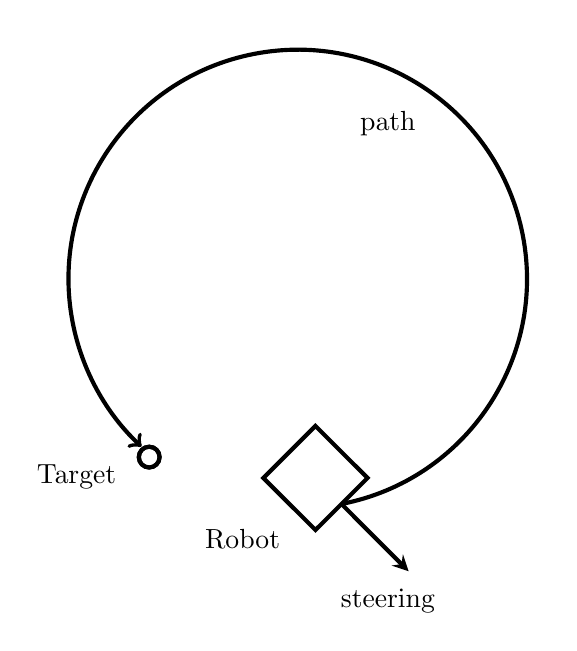
\begin{tikzpicture}
\pgftransformxscale{1.000000}
\pgftransformyscale{-1.000000}
\definecolor{dialinecolor}{rgb}{0.000000, 0.000000, 0.000000}
\pgfsetstrokecolor{dialinecolor}
\definecolor{dialinecolor}{rgb}{1.000000, 1.000000, 1.000000}
\pgfsetfillcolor{dialinecolor}
\pgfsetlinewidth{0.100000\du}
\pgfsetdash{}{0pt}
\pgfsetdash{}{0pt}
\pgfsetbuttcap
{
\definecolor{dialinecolor}{rgb}{0.000000, 0.000000, 0.000000}
\pgfsetfillcolor{dialinecolor}
% was here!!!
\pgfsetarrowsend{stealth}
\definecolor{dialinecolor}{rgb}{0.000000, 0.000000, 0.000000}
\pgfsetstrokecolor{dialinecolor}
\draw (40.907057\du,26.405166\du)--(42.500000\du,28.000000\du);
}
\pgfsetlinewidth{0.100000\du}
\pgfsetdash{}{0pt}
\pgfsetdash{}{0pt}
\pgfsetmiterjoin
\definecolor{dialinecolor}{rgb}{0.000000, 0.000000, 0.000000}
\pgfsetstrokecolor{dialinecolor}
\draw (40.255330\du,24.500000\du)--(41.510660\du,25.752665\du)--(40.255330\du,27.005330\du)--(39.000000\du,25.752665\du)--cycle;
% setfont left to latex
\definecolor{dialinecolor}{rgb}{0.000000, 0.000000, 0.000000}
\pgfsetstrokecolor{dialinecolor}
\node at (40.255330\du,25.947665\du){};
\pgfsetlinewidth{0.100000\du}
\pgfsetdash{}{0pt}
\pgfsetdash{}{0pt}
\pgfsetbuttcap
\pgfsetmiterjoin
\pgfsetlinewidth{0.100000\du}
\pgfsetbuttcap
\pgfsetmiterjoin
\pgfsetdash{}{0pt}
\definecolor{dialinecolor}{rgb}{1.000000, 1.000000, 1.000000}
\pgfsetfillcolor{dialinecolor}
\pgfpathellipse{\pgfpoint{36.250000\du}{25.250000\du}}{\pgfpoint{0.250000\du}{0\du}}{\pgfpoint{0\du}{0.250000\du}}
\pgfusepath{fill}
\definecolor{dialinecolor}{rgb}{0.000000, 0.000000, 0.000000}
\pgfsetstrokecolor{dialinecolor}
\pgfpathellipse{\pgfpoint{36.250000\du}{25.250000\du}}{\pgfpoint{0.250000\du}{0\du}}{\pgfpoint{0\du}{0.250000\du}}
\pgfusepath{stroke}
\pgfsetbuttcap
\pgfsetmiterjoin
\pgfsetdash{}{0pt}
\definecolor{dialinecolor}{rgb}{0.000000, 0.000000, 0.000000}
\pgfsetstrokecolor{dialinecolor}
\pgfpathellipse{\pgfpoint{36.250000\du}{25.250000\du}}{\pgfpoint{0.250000\du}{0\du}}{\pgfpoint{0\du}{0.250000\du}}
\pgfusepath{stroke}
\pgfsetlinewidth{0.100000\du}
\pgfsetdash{}{0pt}
\pgfsetdash{}{0pt}
\pgfsetbuttcap
{
\definecolor{dialinecolor}{rgb}{0.000000, 0.000000, 0.000000}
\pgfsetfillcolor{dialinecolor}
% was here!!!
\pgfsetarrowsend{to}
\definecolor{dialinecolor}{rgb}{0.000000, 0.000000, 0.000000}
\pgfsetstrokecolor{dialinecolor}
\pgfpathmoveto{\pgfpoint{40.882550\du}{26.379091\du}}
\pgfpatharc{79}{-227}{5.522390\du and 5.522390\du}
\pgfusepath{stroke}
}
% setfont left to latex
\definecolor{dialinecolor}{rgb}{0.000000, 0.000000, 0.000000}
\pgfsetstrokecolor{dialinecolor}
\node at (38.500000\du,27.222500\du){Robot};
% setfont left to latex
\definecolor{dialinecolor}{rgb}{0.000000, 0.000000, 0.000000}
\pgfsetstrokecolor{dialinecolor}
\node at (34.500000\du,25.722500\du){Target};
% setfont left to latex
\definecolor{dialinecolor}{rgb}{0.000000, 0.000000, 0.000000}
\pgfsetstrokecolor{dialinecolor}
\node at (42.000000\du,17.222500\du){path};
% setfont left to latex
\definecolor{dialinecolor}{rgb}{0.000000, 0.000000, 0.000000}
\pgfsetstrokecolor{dialinecolor}
\node at (42.000000\du,28.722500\du){steering};
\end{tikzpicture}

    \end{center}
    
    \caption{
        \label{fig:path}
        Path used to reach the target
    }
\end{figure}

\paragraph{}{
    In fact, the way I compute the speeds, and in particular the angular speed
can be improved. Let's say the schema at figure \ref{fig:path} represents what
the robot currently do. The straight arrow presents the steering of the
robot, and the other one stands for the trajectory followed currently by the
robot. As you can notice it could be quicker and smart to turn to the other 
way. To do so, when I compute the angle between the robot and the carrot, I
just have to check if the angle is lower than $-\pi$ or if it is greater than $\pi$, if so, I add\/substrate $2\pi$ to the current angle. That turns the
algorithm to the one at figure \ref{algo:speeds_smart}. Now the robot avoids 
U-turns.
}

\begin{figure}[!h]
    \begin{algorithmic}
     \Function{compute\_speeds}{robot, carrot}
        \State $distance \gets \sqrt{(carrot.x - robot.x)^{2} + (carrot.y - robot.y)^{2}}$
        \State $robot\_angle \gets \Call{getRobotSteering}$
        \State $carrot\_angle \gets \Call{atan2}{carrot.y - robot.x, carrot.x - robot.x}$
        \State $angle = carrot\_angle - robot\_angle$
        \If{ $-\pi > angle$ }
            \State $ angle \gets 2\pi + angle $
        \EndIf
        \If{ $\pi < angle$ }
            \State $ angle \gets 2\pi - angle $
        \EndIf
        \State $angular\_speed = angle / 1$
        \State $linear\_speed \gets angular\_speed \times \frac{distance}{2 \times sin( angle )} $
        \State \Return $linear\_speed,~angular\_speed$
     \EndFunction
    \end{algorithmic}
    
    \caption{
        \label{algo:speeds_smart}
        Algorithm to compute the speed to reach a target point
    }
\end{figure}

\paragraph{}{
}

\paragraph{}{
   Now the robot can follow the path using \textit{Follow the carrot}
 \cite{thesis:barton}. The name of this method is due to the way it processes
 the path points. As you can see, each point are considered. For each point the
 algorithm computes with speeds the robot should use to reach the target point.
 and once it reached it, we repeat the process for the next point. But this
 method has a drawback. It is slow!
}

\paragraph{}{
    Considering each single point of the path is a waste. In fact, trying to
 reach each of them takes a while. And increasing the computed speeds by the
 program is not the right solution because it makes the robot too fast and it
 misses the targeted position: The robot became unstable. So, let's thinking
 about something more \textit{intelligent}, skipping some points. \newline
 The point of the path are very closed, so trying to reach all of them it's
 certainly not the right thing. Skipping \textit{some} points has many
 advantages. Firstly, less point means less computation. It is not critical  
 here, but still it is never a bad thing while the outputs are correct. Then, by
 skipping points, the robot will target points which are more away and so the
 computed speeds will be higher. Then, the path used by the robot is more
 smooth. Finally, the robot is quicker. But how to do it ?
}

\begin{figure}[!h]
    \begin{algorithmic}
        \ForAll{point in path}
            \State $position \gets \Call{getRobotRosition}$
            \State $distance \gets \sqrt{(point.x - robot.x)^{2} + (point.y - robot.y)^{2}}$
            \If{$distance < lookahead$}
                \While{$distance > threshold$}
                    \State $speeds \gets \Call{compute\_speeds(position, point)}$
                    \State $\Call{setSpeeds}{speeds}$
                    \State $position \gets \Call{getRobotRosition}$
                    \State $distance \gets \sqrt{(point.x - robot.x)^{2} + (point.y - robot.y)^{2}}$
                \EndWhile
            \EndIf
        \EndFor
        \State $\Call{setSpeeds}{\{ 0, 0\}}$
    \end{algorithmic}
    
    \caption{
        \label{algo:v2}
        \textit{Follow the carrot} modified algorithm
    }
\end{figure}

\paragraph{Look-ahead distance and threshold}{
    Firstly, to avoid the closest points, I define a look-ahead distance in the
 program. Basically, it is a imaginary circle around the robot. Every points
 (except if it is the last one), in this distance are ignored. That makes the
 robot trajectories more smooth. Then, The robot do not have to sharply come by
 by each targeted point. So, I define a threshold which is the minimum distance
 the robot has to reach before trying to reach another one. Now the obtain the
 algorithm figure \ref{algo:v2}.
}

